\section{Tutorial}\label{sec:ambulance_game_tutorial}

The following tutorial provides the steps to get the Nash
equilibrium of an instance of the game between two hospitals and an ambulance
service provider using the \texttt{ambulance\_game} library.
Table~\ref{tab:ambulance_game_example} provides the parameters of the game
instance.

\begin{table}[H]
    \begin{center}
        \begin{tabular}{||c|c|c|c||}
            \hline
            \(\lambda_2\) & t & \footnotesize{\(\hat{P}\)} & \(\alpha\) \\
            \hline\hline
            8 & 2 & 0.7 & 0.5 \\
            \hline
        \end{tabular}

        \vspace{0.3cm}

        \begin{tabular}{||c|c|c|c|c|c||}
            \hline
            \(\lambda_1^A\) & \(\mu^A\) & \(C^A\) & \(N^A\) & \(M^A\) \\
            \hline\hline
            1 & 3 & 2 & 10 & 5 \\
            \hline
        \end{tabular}

        \vspace{0.3cm}
        
        \begin{tabular}{||c|c|c|c|c|c||}
            \hline
            \(\lambda_1^B\) & \(\mu^B\) & \(C^B\) & \(N^B\) & \(M^B\) \\
            \hline\hline
            2 & 1 & 3 & 10 & 5 \\
            \hline
        \end{tabular}
    \end{center}
    \caption{Parameters of the game}
    \label{tab:ambulance_game_example}
\end{table}

A full description of the parameters of the game can also be found in
Section~\ref{sec:game_players_and_parameters}.
The code snippet in Listing~\ref{lst:abg_tutorial_parameters} defines the
parameters of the game instance using Python.

\begin{lstlisting}[
    style=pystyle,
    caption={Python code that defnies the parameters.},
    label={lst:abg_tutorial_parameters},
]
>>> lambda_2 = 8
>>> target = 2
>>> alpha = 0.5
>>> p_hat = 0.7
>>>
>>> lambda_1_1 = 1
>>> mu_1 = 3
>>> num_of_servers_1 = 2
>>> system_capacity_1 = 10
>>> buffer_capacity_1 = 5
>>>
>>> lambda_1_2 = 2
>>> mu_2 = 1
>>> num_of_servers_2 = 3
>>> system_capacity_2 = 10
>>> buffer_capacity_2 = 5

\end{lstlisting}

The arrival rate of type 2 individuals (ambulance patients) is set to
\texttt{lambda\_2 = 8}.
The parameters that correspond to the policy imposed to the hospitals are
\texttt{target = 2} and \texttt{p\_hat = 0.7}.
This means that the hospitals should aim to serve \(70\%\) of the patients
that arrive at the hospital within \(2\) time units.

The python code shown in~\ref{lst:abg_tutorial_game_instance} uses the
parameters of the current game to create matrices \(A\), \(B\) and \(R\)
that represent the payoff matrices of the game and the routing matrix
respectively.
For more information on the matrices of the game, refer to
Section~\ref{sec:queueing_systems_and_normal_form_games}.
The code snippet also uses the \texttt{nashpy} library~\cite{thenashpyproject}
to define the game object.

\begin{lstlisting}[
    style=pystyle,
    caption={Python code that defines the game instance.},
    label={lst:abg_tutorial_game_instance},
]
>>> import ambulance_game as abg
>>> import numpy as np
>>> import nashpy as nash
>>>
>>> A, B, R = abg.game.get_payoff_matrices(
...     lambda_2=lambda_2,
...     target=target,
...     alpha=alpha,
...     p_hat=p_hat,
...     lambda_1_1=lambda_1_1,
...     lambda_1_2=lambda_1_2,
...     mu_1=mu_1,
...     mu_2=mu_2,
...     num_of_servers_1=num_of_servers_1,
...     num_of_servers_2=num_of_servers_2,
...     system_capacity_1=system_capacity_1,
...     system_capacity_2=system_capacity_2,
...     buffer_capacity_1=buffer_capacity_1,
...     buffer_capacity_2=buffer_capacity_2,
... )
>>> game = nash.Game(A, B)

\end{lstlisting}

Thus, a Nash equilibrium of the game can be found using the
\texttt{lemke\_howson} function of the \texttt{nashpy} library.
The Python code shown in Listing~\ref{lst:abg_tutorial_nash_equilibrium}
gets a Nash equilibrium of the game instance.

\begin{lstlisting}[
    style=pystyle,
    caption={Python code that finds a Nash equilibrium of the game instance.},
    label={lst:abg_tutorial_nash_equilibrium},
]
>>> strat_1, strat_2 = game.lemke_howson(initial_dropped_label=0)
>>> strat_1
array([0., 0., 0., 0., 0., 0., 0., 0., 0., 1.])
>>> strat_2
array([0., 0., 0., 0., 0., 1., 0., 0., 0., 0.])

\end{lstlisting}

This corresponds to player \(1\) playing a strategy of
\(\sigma^A = (0, 0, 0, 0, 0, 0, 0, 0, 0, 1)\) and player \(2\) playing a
strategy of \(\sigma^B = (0, 0, 0, 0, 0, 1, 0, 0, 0, 0)\).
This in turn corresponds to player \(1\) choosing a threshold of \(T^A = 10\)
and player \(2\) choosing a threshold of \(T^B = 6\).

Apart from the Nash equilibrium, a learning algorithm can also be used to get
an evolutionary stable strategy (ESS) of the game.
In the code snippet shown in Listing~\ref{lst:abg_tutorial_ard}, the results
of the asymmetric replicator dynamics algorithm run are shown.
The code snippet also uses the \texttt{matplotlib} library to plot the
results of the algorithm.


\definecolor{invisiblecomments}{RGB}{253, 246, 220}
\begin{lstlisting}[
    style=pystyle,
    caption={Python code that runs the asymmetric replicator dynamics algorithm.},
    label={lst:abg_tutorial_ard},
    commentstyle=\color{invisiblecomments},
    showstringspaces=false,
]
>>> import matplotlib.pyplot as plt
>>> xs,ys = game.asymmetric_replicator_dynamics(
...     timepoints=np.linspace(0, 10000, 1000)
... )
>>>
>>> plt.plot(xs[0:30]) # doctest: +SKIP
>>> plt.title("Asymmetric replicator dynamics for player 1") # doctest: +SKIP
>>> plt.xlabel("Timepoints") # doctest: +SKIP
>>> plt.ylabel("Probability") # doctest: +SKIP
>>>
>>> plt.plot(ys) # doctest: +SKIP
>>> plt.title("Asymmetric replicator dynamics for player 2") # doctest: +SKIP
>>> plt.xlabel("Timepoints") # doctest: +SKIP
>>> plt.ylabel("Probability") # doctest: +SKIP
    
\end{lstlisting}

\begin{figure}[H]
    \centering
    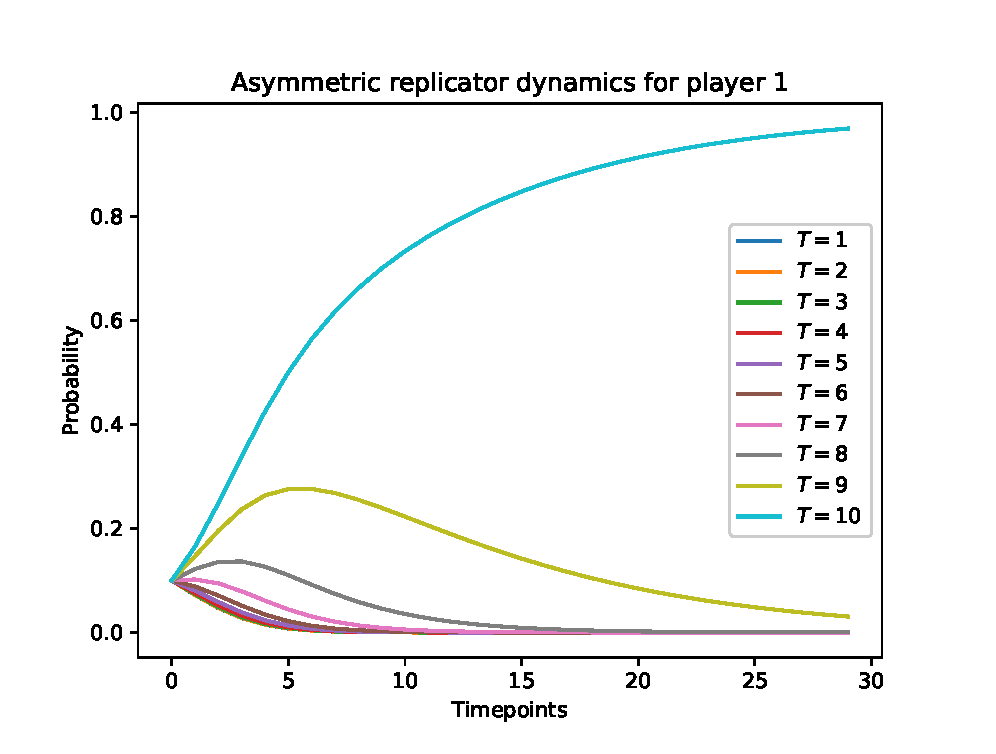
\includegraphics[width=0.49\textwidth]{chapters/00_appendix/01_ambulance_game_library/Bin/ard_p1.eps}
    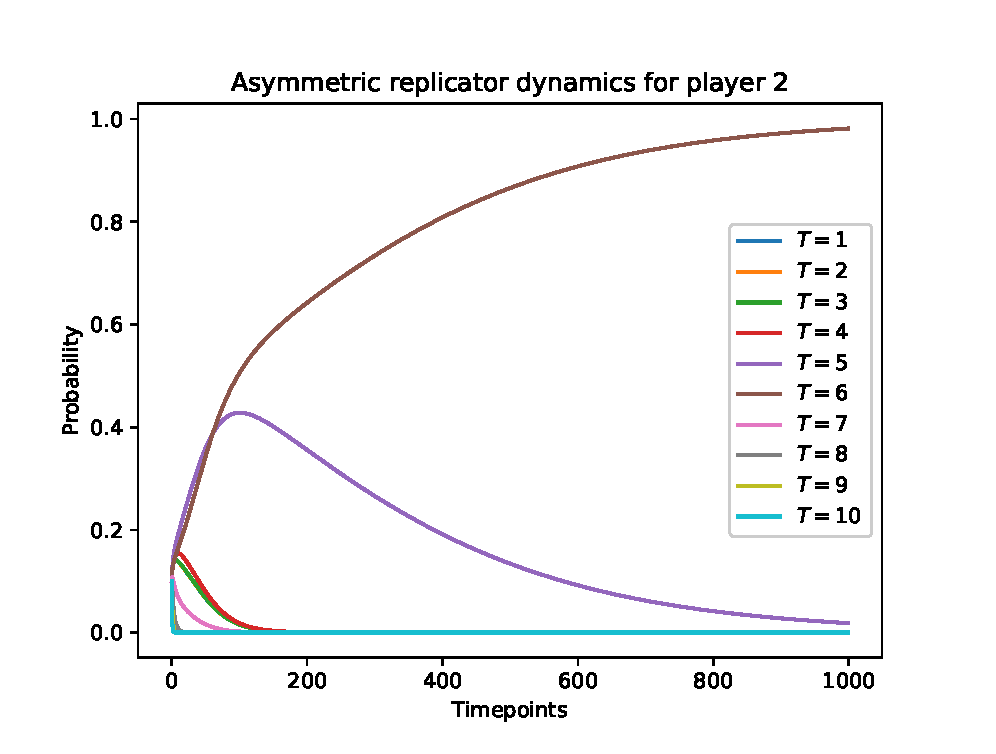
\includegraphics[width=0.49\textwidth]{chapters/00_appendix/01_ambulance_game_library/Bin/ard_p2.eps}
\end{figure}


From the results of both the Lemke-Howson algorithm and the asymmetric
replicator dynamics algorithm, the same pair of strategies is found.
That is player \(1\) choosing a threshold of \(T^A = 10\) and player \(2\)
choosing a threshold of \(T^B = 6\).
The equivalent strategy of the third player; the ambulance service, can be
found from the routing matrix \(R\) in position \(R_{10, 6}\).


\begin{lstlisting}[
    style=pystyle,
    caption={Python code for the strategy of the third player.},
    label={lst:abg_tutorial_routing_strategy},
]
>>> threshold_1, threshold_2 = 10, 6
>>> prop_A = R[threshold_1 - 1, threshold_2 - 1]
>>> prop_B = 1 - prop_A
>>> np.round(prop_A, 2), np.round(prop_B, 2)
(0.95, 0.05)

\end{lstlisting}

In response to the thresholds chosen by the first two players, the ambulance
service chooses to send \(95\%\) of the ambulances to the first hospital and
\(5\%\) of the ambulances to the second hospital.
Having this percentage of ambulances sent to each hospital, the overall waiting
time of patients at each hospital can be calculated.
The Python code shown in Listing~\ref{lst:abg_tutorial_waiting_time} calculates
the waiting time of patients at each hospital.

\begin{lstlisting}[
    style=pystyle,
    caption={Python code for the waiting time of patients at each hospital.},
    label={lst:abg_tutorial_waiting_time},
]
>>> mean_wait_1 = abg.markov.get_mean_waiting_time_using_markov_state_probabilities(
...     lambda_2=lambda_2 * prop_A,
...     lambda_1=lambda_1_1,
...     mu=mu_1,
...     num_of_servers=num_of_servers_1,
...     threshold=threshold_1,
...     system_capacity=system_capacity_1,
...     buffer_capacity=buffer_capacity_1,
... )
>>> mean_wait_2 = abg.markov.get_mean_waiting_time_using_markov_state_probabilities(
...     lambda_2=lambda_2 * (1 - prop_A),
...     lambda_1=lambda_1_2,
...     mu=mu_2,
...     num_of_servers=num_of_servers_2,
...     threshold=threshold_2,
...     system_capacity=system_capacity_2,
...     buffer_capacity=buffer_capacity_2,
... )
>>> np.round(mean_wait_1, 3)
1.257
>>> np.round(mean_wait_2, 3)
0.632

\end{lstlisting}

The results of the calculations show that the average waiting time of patients
at the first hospital is \(1.257\) time units and the average waiting time of
patients at the second hospital is \(0.632\) time units.
Going back to the parameters that relate to the policy imposed on the hospitals,
\texttt{target = 2} and \texttt{p\_hat = 0.7}.
As stated earlier, that corresponds to both hospitals serving \(70\%\) of the
patients within \(2\) time units.
The mean total time of patients is calculated by adding the average waiting
time and the average service time of patients.

\begin{lstlisting}[
    style=pystyle,
    caption={Python code for the mean total time of patients at each hospital.},
    label={lst:abg_tutorial_mean_total_time},
]
>>> np.round(mean_wait_1 + (1 / mu_1), 3)
1.591
>>> np.round(mean_wait_2 + (1 / mu_2), 3)
1.632
    
\end{lstlisting}

The first mean time in hospital \(1\) for patients is \(1.591\) time units and
the mean time in hospital \(2\) for patients is \(1.632\) time units.
